% Create a document for a project proposal
\documentclass[11pt]{article}
% Packages
\usepackage{geometry}
\geometry{
    top=1.5cm,
    bottom=1.5cm,
    left=2cm,
    right=2cm
}
\usepackage{ragged2e}
\usepackage{algorithm}
\usepackage{algpseudocode}
\usepackage{graphicx}
\usepackage{tikz}
% Options for packages loaded elsewhere
\PassOptionsToPackage{unicode}{hyperref}
\PassOptionsToPackage{hyphens}{url}
\usepackage{amsmath,amssymb}
\usepackage{lmodern}
\usepackage{iftex}
\ifPDFTeX
    \usepackage[T1]{fontenc}
    \usepackage[utf8]{inputenc}
    \usepackage{textcomp} % provide euro and other symbols
\else % if luatex or xetex
    \usepackage{unicode-math}
    \defaultfontfeatures{Scale=MatchLowercase}
    \defaultfontfeatures[\rmfamily]{Ligatures=TeX,Scale=1}
\fi
% Use upquote if available, for straight quotes in verbatim environments
\IfFileExists{upquote.sty}{\usepackage{upquote}}{}
\IfFileExists{microtype.sty}{% use microtype if available
    \usepackage[]{microtype}
    \UseMicrotypeSet[protrusion]{basicmath} % disable protrusion for tt fonts
}{}
\makeatletter
\@ifundefined{KOMAClassName}{% if non-KOMA class
    \IfFileExists{parskip.sty}{%
        \usepackage{parskip}
    }{% else
        \setlength{\parindent}{0pt}
    \setlength{\parskip}{6pt plus 2pt minus 1pt}}
}{% if KOMA class
\KOMAoptions{parskip=half}}
\makeatother
\usepackage{xcolor}
\setlength{\emergencystretch}{3em} % prevent overfull lines
\providecommand{\tightlist}{%
\setlength{\itemsep}{0pt}\setlength{\parskip}{0pt}}
\setcounter{secnumdepth}{-\maxdimen} % remove section numbering
\newlength{\cslhangindent}
\setlength{\cslhangindent}{1.5em}
\newlength{\csllabelwidth}
\setlength{\csllabelwidth}{3em}
\newlength{\cslentryspacingunit} % times entry-spacing
\setlength{\cslentryspacingunit}{\parskip}
\newenvironment{CSLReferences}[2] % #1 hanging-ident, #2 entry spacing
{% don't indent paragraphs
    \setlength{\parindent}{0pt}
    % turn on hanging indent if param 1 is 1
    \ifodd #1
        \let\oldpar\par
        \def\par{\hangindent=\cslhangindent\oldpar}
    \fi
    % set entry spacing
    \setlength{\parskip}{#2\cslentryspacingunit}
}%
{}
\usepackage{calc}
\newcommand{\CSLBlock}[1]{#1\hfill\break}
\newcommand{\CSLLeftMargin}[1]{\parbox[t]{\csllabelwidth}{#1}}
\newcommand{\CSLRightInline}[1]{\parbox[t]{\linewidth - \csllabelwidth}{#1}\break}
\newcommand{\CSLIndent}[1]{\hspace{\cslhangindent}#1}
\ifLuaTeX
    \usepackage{selnolig}  % disable illegal ligatures
\fi
\IfFileExists{bookmark.sty}{\usepackage{bookmark}}{\usepackage{hyperref}}
\IfFileExists{xurl.sty}{\usepackage{xurl}}{} % add URL line breaks if available
\urlstyle{same} % disable monospaced font for URLs
\hypersetup{
    hidelinks,
pdfcreator={LaTeX via pandoc}}

% Title
\title{\textbf{Design \& Analysis of Algorithms Proposal \\ \vspace{5mm} EEG classification using Deep Learning Algorithms}}
\author{\textbf{Team Members} \vspace{1mm} \\ Muhammad Athar (408369) \\ Muhammad Arsalan Khan (410963) \vspace{5mm} \\ \textbf{Class: }BESE - 13A}

\begin{document}
\maketitle

\justifying
\section{Introduction}
The semester project for Design and Analysis of Algorithms aims to tackle the problem of classifying EEG (Electroencephalography) files as either normal or abnormal.
Electroencephalography (EEG) is a non-invasive method used to record electrical activity of the brain. However, manual analysis of EEG data is time consuming and requires expertise of highly trained neurologists. Unfortunately, there is a lack of clinically certified neurologists in developing countries especially in Pakistan. Therefore, the aim of this project is to develop a deep learning model that can classify EEG files as either normal or abnormal. Such deep learning model would help in the initial screening of EEG files and would reduce the workload of neurologists.

\subsection{Timeline}
The project is estimated to take a further of 2-3 months to be completely finalized. However, our first model of SCNet had been prepared and trained upon.
The timeline for the project is as follows:

\begin{center}
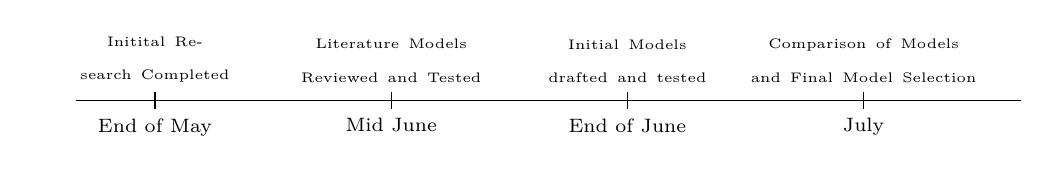
\begin{tikzpicture}
        
\draw (0,0) -- (12,0);
\foreach \x in {1,4,7,10}
    \draw (\x cm,3pt) -- (\x cm,-3pt);


% Adding All the events
\draw (1,0) node[below=3pt] {\scriptsize End of May} node[above=3pt, text width=3cm, align=center] {\tiny Initital Research Completed};
\draw (4,0) node[below=3pt] {\scriptsize Mid June} node[above=3pt, text width=3cm, align=center] {\tiny Literature Models Reviewed and Tested};
\draw (7,0) node[below=3pt] {\scriptsize End of June} node[above=3pt, text width=3cm, align=center] {\tiny Initial Models drafted and tested};
\draw (10,0) node[below=3pt] {\scriptsize July} node[above=3pt, text width=3cm, align=center] {\tiny Comparison of Models and Final Model Selection};


\end{tikzpicture}
\end{center}

\begin{itemize}
    \item \textbf{End of May:} The initital research on EEG Classification using deep learning technique is already complete.
    \item A single model has also been prepared in tensorflow replicating the SCNet implementation.
    \item \textbf{June Beginning:} At the start of june, most models that are present in the literature will be replicated and tested locally on multiple datasets.
    \item \textbf{Mid June:} New implementations of the model will be finalized and worked upon. They will also be tested on multiple datasets.
    \item \textbf{End of June:} The models will be compared to find the best performing models and to evaluate the results.
\end{itemize}

\section{Contribution}












The project will be divided into the following steps:
\begin{enumerate}
    \item Data Collection: Collect EEG files from publicly available datasets.
    \item Data Preprocessing: Preprocess the EEG files to remove noise and artifacts.
    \item Feature Extraction: Extract features from the EEG files using Convolutional Neural Networks (CNNs).
    \item Model Training: Train the model using the extracted features.
    \item Model Evaluation: Evaluate the model using various metrics like accuracy, F1-Score, and G-mean.
\end{enumerate}

\section{Literature Review}
There have been many studies that have used various machine learning algorithms to classify EEG files like AlexNet followed by Support Vector Machines(SVMs). A recent study published in 2023 used a novel model for the classification of EEGs which was named SCNet (Spatial Feature Fused Convolutional Network) which has been able to achieve an accuracy of 90.57\% and has also performed well in other metrics like F1-Score and G-mean. (Wu et al., 2023)

\section{Proposed Methodology}
Based on the above literature review, we have decided to go with the SCNet model for the classification of EEG files, as it is both light-weight (having only about 45,000 parameters), and due to its high accuracy in performing the classification of EEG files into normal and abnormal. (Wu et al., 2023)

\begin{algorithm}
    \caption{SCNet Algorithm}
    \begin{algorithmic}[1]
        \Procedure{Classify}{Raw EEG} \Comment{The Raw EEG is input}
        \State Total Channels $\gets 21$
        \State Input Format: EEG data Channels $[e_i]$ where $i \gets 0$ to $21$
        \State $e_i \gets [e_j]$ where $j \gets 0$ to $n$ where $n$ is the number of timestamps
        \State 
        \State Output Format: Class of the EEG in binary (Abnormal/Normal)
        \State

        \State Output $\gets$ \Call{Preprocess}{Raw EEG} \Comment{Preprocess the Raw EEG}
        \State Output $\gets$ \Call{SpatialFeatures}{Output}
        \State Output $\gets$ \Call{TemporalFeatures}{Output}
        \State Class $\gets$ \Call{Classify}{Output}
        \State \textbf{return} Class\Comment{Returns the class of the classified EEG}
        \EndProcedure
    \end{algorithmic}
\end{algorithm}

\begin{algorithm}
    \caption{Temporal Net Algorithm}
    \begin{algorithmic}[1]
        \Procedure{Classify}{Raw EEG} \Comment{The Raw EEG is input}
        \State Total Channels $\gets 21$
        \State Input Format: EEG data Channels $[e_i]$ where $i \gets 0$ to $21$
        \State $e_i \gets [e_j]$ where $j \gets 0$ to $n$ where $n$ is the number of timestamps
        \State 
        \State Output Format: Class of the EEG in binary (Abnormal/Normal)
        \State

        \State Output $\gets$ \Call{Preprocess}{Raw EEG} \Comment{Preprocess the Raw EEG}
        \State Output $\gets$ \Call{TemporalFeatures}{Output}
        \State Class $\gets$ \Call{Classify}{Output}
        \State \textbf{return} Class\Comment{Returns the class of the classified EEG}
        \EndProcedure
    \end{algorithmic}

\end{algorithm}


\begin{algorithm}
    \caption{Feature Extraction using CNNs}
    \begin{algorithmic}[1]
        \Procedure{Features}{raw}
        \State Input Format: $[e_{ij}]$ where $i \gets 0$ to $h_0$ and $j \gets 0$ to $w_0$
        \State Output Format: $[e_{ijk}]$ where $i \gets 0$ to $h_1$, $j \gets 0$ to $w_1$ and $k \gets 0$ to $d$

        \Comment Depth is an extra dimension in the output due to multiple features
        \State $w \gets width$, $h \gets height$ and $d \gets depth$
        \State Apply Kernels on $[e_{xy}] \in [e_{ij}]$ 

        \State \Comment Kernels are applied on the input data
        \State $[e_{ij}]_0 = [w_{ij}] * [e_{ij}] + b$
        \State \Comment Kernels multiply weights to each element in the data and add bias
        \State $[e_{ijk}] \gets$ \textbf{concat}($[e_{ij}]_y$) \Comment Concatenate on z-axis
        \State \Comment These outputs are represented in the output matrix

        \State \textbf{return} $[e_{ijk}]$


        \EndProcedure

    \end{algorithmic}
\end{algorithm}

\newpage
\section{Conclusion}
In conclusion, the SCNet model has been chosen for the classification of EEG files as it has shown to be effective in classifying EEG files into normal and abnormal. The model is light-weight and has a high accuracy of 90.57\%. (Wu et al., 2023)

\section{Reference}
\hypertarget{refs}{}
\begin{CSLReferences}{1}{0}
    \leavevmode\vadjust pre{\hypertarget{ref-WU2023105059}{}}%
    Wu, Tao, Yujie Fan, Yunning Zhong, Xiu Cheng, Xiangzeng Kong, and Lifei
    Chen. 2023. {``SCNet: A Spatial Feature Fused Convolutional Network for
    Multi-Channel EEG Pathology Detection.''} \emph{Biomedical Signal
    Processing and Control} 86: 105059.
    \url{https://doi.org/10.1016/j.bspc.2023.105059}.

\end{CSLReferences}

\end{document}
